\begin{figure*}[t]
  \centering
  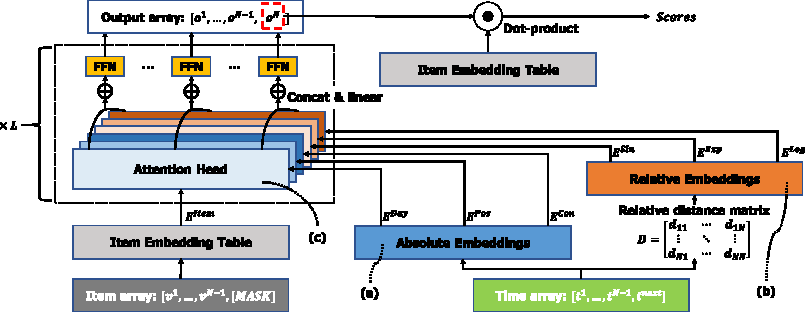
\includegraphics[width=0.9\linewidth]{figures/model_figure.pdf}
  \caption{Model Architecture}
  \Description[The figure describes our model architecture.]{In the figure, item array is converted by item embedding table and fed to each attention head. Time array is converted by absolute/relative embeddings into 6 different embeddings. Each attention head receives item embedding and unique temporal embedding. Concat&linear and FFN operation lies above the heads. Heads and FFNs are repeated for L layers. At the end of the layer, output vector is dot-producted with item embedding table to compute the final item score distribution.}
  \label{fig:model}
\end{figure*}

\begin{figure*}[t]
  \centering
  
\includegraphics[width=\linewidth]{figures/attention.pdf}
  \caption{Brief overview of single attention head in multi-headed attention structure. (a) absolute self-attention in Transformer (b) relative self-attention in Transformer-XL and MEANTIME (c) absolute self-attention in MEANTIME.}
  \Description[The figure describes three different types of single attention-head]{Figure(a) describes a single attention head used in transformer. The sum of E^Item and E^Pos is fed to the head. Figure(b) describes a single attention head from Transformer-xl and our model. E^Pos is replaced by E^R and positional information is not used in value computation. Linear layers are also separated between content and position. Figure(c) describes a single attention head used for absolute attention in our model. It borrows the structure from (a), but separates the content and position as in (b).}
  \label{fig:attntypes}
\end{figure*}

Several self-attention based recommendation models have been proposed recently~\cite{SASRec, BERT4Rec}. However, the positional factors have been rather overlooked in these models for many reasons. First, they don't utilize timestamp values which hold important contextual information. While TiSASRec~\cite{TISASRec} successfully addressed this issue, they also used a simple embedding scheme for temporal values. This can possibly lead to an information bottleneck since the same embedding has to represent all possible positional biases. Furthermore, since all attention heads use the same positional information, they might wastefully learn the same patterns. As a way to mitigate these problems, we devise a novel model architecture that injects various temporal embeddings for each attention head as shown in Figure \ref{fig:model}.

\subsection{Problem Formulation}
%Let $U=\{u_1,u_2,…,u_{|U|}\}$ be a set of users, and $V=\{v_1,v_2,…,v_{|V|}\}$ be a set of items. For each user $u \in U$, we have a sequence of items that the user interacted with in the past, denoted by $S_u=[v_1^{(u)},…,v_k^{(u)},…,v_{|S_u|}^{(u)}]$ where $v_k^{(u)}$ is the $k^{th}$ interacted item in chronological order. We also assume that each interaction is tagged by a positive integer which represents the absolute timestamp of the interaction (e.g. unix timestamp). Therefore each sequence $S_u$ has a corresponding time sequence $T_u=[t_1^{(u)},…,t_k^{(u)},…,t_{|S_u|}^{(u)}]$ where $t_k^{(u)}$ is the timestamp of $v_k^{(u)}$. Given an interaction history $(S_u,T_u)$ and a target timestamp $t_{|S_u |+1}^{(u)}$, our goal is to predict the next item that the user is likely to interact with at the target timestamp. This can be done by modeling the probability  $p\Big(v_{|S_u |+1}^{(u)} = v \Big| S_u,T_u \Big)$ over a set of candidate items for the user $u$ at timestamp $t_{|S_u|+1}^{(u)}$. 


Let $U$ be a set of users, and $V$ a set of items. For each user $u\in U$, we have a sequence of items $V^u=[v^u_1, ..., v^u_k, ..., v^u_{|V^u|}|v^u_k\in V]$ that the user previously interacted with in chronological order and the corresponding time sequence of the interaction $T^u=[t^u_1, ..., t^u_k, ..., t^u_{|V^u|}|t^u_k\in \mathbb{N}]$ that stores the absolute timestamp values.
%e.g., unix timestamp.
Our goal is to predict the next item $v^u_{next}$ that the user $u$ is likely to interact with at the target timestamp $t^u_{next}$ based on the given history $(V^u, T^u)$. % This can be done by modeling the probability  $p\Big(v_{|S_u |+1}^{(u)} = v \Big| S_u,T_u \Big)$ over a set of candidate items for the user $u$ at timestamp $t_{|S_u|+1}^{(u)}$. 

\sloppy Our model is based on a fixed-length model with length $N$ as in previous works~\cite{SASRec, BERT4Rec}. Given the history $(V_u, T_u)$ of user $u$, we feed $\mathbf{v} = [v^u_{|V^u|-N+2}, ..., v^u_{|V^u|}, \text{[MASK]}]$ and $\mathbf{t} = [t^u_{|V^u|-N+2}, ..., t^u_{|V^u|}, t^u_{next}]$ to the model. Then the model estimates $v_{next}$ as output. If the history is shorter than $N-1$, it is padded by a special token [PAD]. 


\subsection{Input Embedding}
\label{section:inputembedding}
The embedding layers convert $\mathbf{v}$ and $\mathbf{t}$ to hidden features that are provided to the attention module. In the case of item array $\mathbf{v}$, each element has an item index. This array is embedded as $E^{item} \in \mathbb{R}^ {N\times h}$ using the conventional look-up operation with a learnable item embedding table $M^I\in \mathbb{R}^{(|V|+1)\times h}$, where h is the hidden feature size. $M^I$ holds embeddings for $|V|$ items and [MASK] token.

In the case of $\mathbf{t}$, each element has a timestamp value.
%While previous studies~\cite{SASRec, BERT4Rec} use them only to impose an order on the sequence, these values actually hold a lot of information. For instance, temporal difference between two interactions is highly related to the influence they have on each other.
In previous studies, these values were embedded in a single embedding scheme, if they were used at all. However, given that user's behaviors are mixed with various patterns, a single embedding might not suffice. Moreover, using different encoding functions (instead of plain learnable values) for each embedding is beneficial since we can train each of them to learn a unique pattern. With these in mind, we propose six methods to embed $\mathbf{t}$: three absolute methods (Figure \ref{fig:model}(a)), and three relative methods (Figure \ref{fig:model}(b)).

Absolute embeddings encode each position in the sequence as $E^{Day}, E^{Pos}\text{, or } E^{Con} \in \mathbb{R}^{N \times h}$. The first is $\textbf{Day}$-embedding which converts the day of each timestamp into an embedding vector to get $E^{Day}$. We keep a learnable embedding matrix $M^D\in R^{|D|\times h}$ where $|D|$ is the number of possible days in the span of the dataset. In our analysis, $\textbf{Day}$ is a reasonable choice of time length considering the trade-off between matrix size and the effectiveness. $\textbf{Pos}$-embedding is analogous to the learnable positional embedding used in~\cite{BERT, BERT4Rec}, where each position has a corresponding embedding in $M^P\in R^{N\times h}$. We convert each position to get $E^{Pos}$. Note that in this case, the embeddings depend only on the indices of time array and not on the timestamp values. \textbf{Con}-embedding is similar to \textbf{Pos}-embedding, except that all position vectors are shared ($M^C\in R^{1\times h}$) to remove positional bias. Hence, $E^{Con}$ is a stack of repeated vectors.

Relative embeddings encode the relationship between each interaction pair in the sequence as $E^{Sin}, E^{Exp}\text{, or } E^{Log} \in \mathbb{R}^{N \times N \times h}$ by utilizing the temporal difference information. First, we define a matrix of temporal differences $\mathbf{D} \in \mathbb{R}^{N \times N}$ whose element is defined as $d_{ab} = (\mathbf{t}_a-\mathbf{t}_b)/\tau$, where $\tau$ is an adjustable unit time difference. We introduce three encoding functions for \textbf{D}.
%that capture different characteristics of these time intervals.
First, $\textbf{Sin}$ encoder converts the difference $d_{ab}$ to a hidden vector $\vec{\theta}_{ab} \in \mathbb{R}^{1 \times h}$, by the following equation:
\begin{equation}
    \vec{\theta}_{ab, 2c} = sin(\frac{d_{ab}}{freq^{\frac{2c}{h}}})\qquad\vec{\theta}_{ab, 2c+1} = cos(\frac{d_{ab}}{freq^{\frac{2c}{h}}})
\end{equation}
where $\vec{\theta}_{ab, c}$ is the $c^{th}$ value of the vector $\vec{\theta}_{ab}$ and $freq$ is an adjustable parameter.
%By applying the encoder function to $\mathbf{D}$, we get $E^{sinusoid} \in R^{N \times N \times h}$ as output.
Likewise, $\textbf{Exp}$ encoder and $\textbf{Log}$ encoder converts $d_{ab}$ to $\vec{e}_{ab}$ and $\vec{l}_{ab}$ respectively by applying the following equations:
\begin{equation}
  \vec{e}_{ab, c} = exp(\frac{-|d_{ab}|}{freq^{\frac{c}{h}}}) \qquad
  \vec{l}_{ab, c} = log(1 + \frac{|d_{ab}|}{freq^{\frac{c}{h}}})
\end{equation}
Stacking these vectors gives us $E^{Sin}, E^{Exp}$ and $E^{Log}$ respectively.

Each embedding offers a distinctive view on temporal data. For example, $\textbf{Sin}$ captures periodic occurrences. Larger time gap is either quickly decayed to zero in $\textbf{Exp}$ or manageably increased in $\textbf{Log}$. $\textbf{Day}$ can confine the attention scope within the same (or similar) day. $\textbf{Pos}$ can pick up the patterns learnt by the previous models. Finally, $\textbf{Con}$ removes positional bias altogether so that the attention can focus only on the relationship between items. These distinctive views enable our self-attention heads (Figure \ref{fig:model}(c)) to attend to different characteristics of the sequence.

\subsection{Self-Attention Structure}
\subsubsection{Attention Architecture}
Multi-head self-attention proposed in Transformer~\cite{TRANSFORMER} shows excellent performance in recommendation tasks~\cite{BERT4Rec}. MEANTIME is also based on this structure. Traditionally, self-attention based models~\cite{SASRec, BERT, BERT4Rec} employ a simple absolute positional encoding by feeding the sum of $E^{Item}$ and $E^{Pos}$ as input as shown in Figure \ref{fig:attntypes}(a). Advanced transformers~\cite{TRANSFORMER-XL, XLNET} enhanced this as shown in Figure \ref{fig:attntypes}(b). $E^{Pos}$ is replaced by the relative positional embedding $E^R$ that only depends on the difference between the positional indices of the array, and positional information is no longer used at key and value encoder. Parameters $b_I$ and $b_R$ serve as global content/positional bias respectively. For absolute embedding, we also adopt the previous structure. In addition, we propose separating the item and positional embedding for absolute attention as shown in Figure \ref{fig:attntypes}(c).
%We also exploit this structure for our relative attention, but use the proposed $E^{Sin},E^{Exp},E^{Log}$ instead of $E^R$. For absolute attention, we separate the query and key embeddings for the item and temporal information as shown in Figure (c). 

As explained in section \ref{section:inputembedding}, we can diversify the positional information that is fed to the attention module. MEANTIME utilizes 3 absolute embeddings and 3 relative embeddings. When fed a relative embedding, the head will operate as in Figure \ref{fig:attntypes}(b) with either $E^{Sin},E^{Exp}\text{ or }E^{Log}$ as input to $K_R$. When fed an absolute embedding, the head will operate as in Figure \ref{fig:attntypes}(c) with either $E^{Day},E^{Pos}\text{ or }E^{Con}$ as input to $Q_A\text{ and } K_A$.
%In total, MEANTIME utilizes $n$ positional embeddings and $n$ attention heads.
As in previous works, the dimension of each head is $\frac{h}{n}$. The choice of $n$ and embedding types are adjustable with regards to the characteristics of the dataset.


%Given a stack of queries, keys, and values as $Q, K$, and $V$, Transformer \cite{TRANSFORMER} applies the following multi-headed attention:
%\begin{equation}
%\label{eq:attn}
%\begin{split}
%    \text{MultiHead}(Q, K, V) &= \text{Concat}(\text{head}_1, ..., \text{head}_n)W^O
%    \\
%    \text{where } \text{head}_i &= \text{Attention}(QW^Q_i, KW^K_i, VW^V_i)
%    \\
%    \text{and } \text{Attention}(Q, K, V) &= \text{softmax}(\frac{QK^T}{\sqrt{d_k}})V
%\end{split}
%\end{equation}
%where $W^Q_i \in \mathbb{R}^{h \times d_q}, W^K_i \in \mathbb{R}^{h \times d_k}, W^V_i \in \mathbb{R}^{h \times d_v}, W^O \in \mathbb{R}^{nd_v \times h}$ are linear projection matrices, $n$ is the number of heads, and $d_q, d_v, d_k$ are the query, key, value dimensions. Usually $d_q = d_v = d_k = \frac{h}{n}$.












%Traditional self-attention based models \cite{SASRec, BERT, BERT4Rec} employ a simple positional encoding where $X + P \in \mathbb{R}^{N \times h}$ is fed to the first transformer layer as in Figure-\ref{fig:attntypes}-(a). $X$ represents \textit{content} (embedding of each word/item) and $P$ represents \textit{position} (absolute embedding of each position).
%More recent transformers \cite{TRANSFORMER-XL, XLNET} enhanced the above by separating content and position, and relying on relative positional information as in Figure-\ref{fig:attntypes}-(b). Notice that positional information is no longer a part of the value $V$. Moreover, absolute positional embedding $P$ is replaced by relative positional embedding $R$ which applies sinusoid encoding to the distance between two positions. Also, separate linear layers $W^{Q_X}_i, W^{K_X}_i, W^{K_X}_i$ are applied to content and positional information. $u$ and $v$ serve as global content/positional bias respectively.

%We observe that in both cases, the same type of positional embedding is used for each head. However, in the case of sequential recommendation, we can diversify the positional embeddings as we showed in \ref{section:inputembedding}. MEANTIME utilizes $n$ positional embeddings and $n$ attention heads. Each head will be fed a different positional embedding. When fed a relative embedding, the head will operate as in Figure-\ref{fig:attntypes}-(b). When fed an absolute embedding, the head will operate as in Figure-\ref{fig:attntypes}-(c), which is a slight variation of Figure-\ref{fig:attntypes}-(a) that adopts recent improvements. The choice of $n$ and embedding types are adjustable with regards to the characteristics of the dataset.


%We make three observations here. First, since $X$ and $P$ are given as a mixed input, they have to share the same linear layers. Furthermore, $P$ is also included in values, which could be undesirable because output should only be about content. Second, since content and positional information is mixed even more in the attention, there is no way to inject positional biases after the first Transformer layer. Third, the above uses the same type of positional embedding for every head. However, we can diversify the positional embedding so that each head gets a different positional bias. This is even more so in the case of sequential recommendation where we can also use time information to create a more well-informed positional embedding.

% To address the above isseus, we devise a different attention operation for our model as follows:
% \begin{equation}
% \text{Attention}(Q, K, V, P) = \text{softmax}\left(\frac{(XW^{Q_X}_i + PW^{Q_P}_i)(XW^{K_X}_i + PW^{K_P}_i)^T}{\sqrt{d_k}}\right)(XW^{V_X}_i)
% \end{equation}

% Notice that our attention takes $P$ as an additional input. This enables our multi-head attention to feed different positional biases for each head, e.g. $E^{Day}, E^{Pos}, E^{Const}$.

% Given an input sequence $\mathbf{X} \in \mathbb{R}^{N \times h}$, a single attention head $\mathbf{B}$ produces an output sequence $\mathbf{Z} \in \mathbb{R}^{N \times h}$. Together with $\mathbf{X}$, the block is given an embedding matrix $\mathbf{E}$ that encodes positional information. $\mathbf{E}$ can either be an absolute position embedding (in which case $\mathbf{E} \in \mathbb{R}^{N \times h}$) or relative position embedding (in which case $\mathbf{E} \in \mathbb{R}^{N \times N \times h}$). The block is called \textbf{Absolute Self-Attention Block} in the former case, and \textbf{Relative Self-Attention Block} in the latter case. We explain both cases in parallel since most operations overlap.

% To compute $\mathbf{Z}$, we define two operations. The first operation is \textbf{MH} (Multi-Headed Self-Attention). We first define \textbf{Self-Attention} as follows:
% \begin{equation}
%   \textbf{Self-Attention}(X, E) = \sum_{j=1}^{n}{attn_{ij} X_j W_{content}^V}
% \end{equation}
% where $W_{content}^V \in \mathbb{R}^{h \times d_v}$ is a learnable linear projection matrix for content values, $d_v$ is the dimension of values, and $attn_{ij} \in \mathbb{R}$ is an attention score. Note that unlike previous works \cite{SASRec, TISASRec, BERT, BERT4Rec}, we are able to exclude any positional information and only consider content information when computing values. We prove that such prevention of information mix-up is beneficial for performance in the ablation study below.

% We compute $attn_{ij}$ as:
% \begin{equation}
%   attn_{ij} = \frac{\exp{\alpha_{ij}}}{\sum_{k=1}^{n}{\exp{\alpha_{ik}}}}
% \end{equation}
% The computation of $\alpha_{ij}$ differs between \textbf{Absolute Self-Attention Block} and \textbf{Relative Self-Attention Block}.

% In the first case,
% \begin{equation}
%   \alpha_{ij} = \frac{ (X_i W_{content}^Q + E_i W_{position}^Q)  (X_j W_{content}^K + E_j W_{position}^K)  }{\sqrt{d_k}}
% \end{equation}
% where $W_{content}^Q \in \mathbb{R}^{h \times d_q}, W_{content}^K \in \mathbb{R}^{h \times d_k}$ are learnable linear projection matrices for content queries and keys, and $W_{position}^Q \in \mathbb{R}^{h \times d_q}, W_{position}^K \in \mathbb{R}^{h \times d_k}$ are learnable linear projection matrices for position queries and keys. $d_q, d_k$ are dimensions of queries and keys. Usually, $d_q = d_k = d_v$ in self-attention. To prevent gradient vanishing or exploding, we scale the score with $\sqrt{d_k}$.

% In the case of \textbf{Relative Self-Attention Block}, $\alpha_{ij}$ is computed as follows:
% \begin{equation}
%   \alpha_{ij} = \frac{ X_i W_{content}^Q  (X_j W_{content}^K + E_{ij} W_{position}^K) +
%                       B_{content} X_j W_{content}^K +
%                       B_{position} E_{ij} W_{position}^K }{\sqrt{d_k}}
% \end{equation}
% where $B_{content}, B_{position} \in \mathbb{R}^{d_q}$ are learnable biases for content and position respectively, and the rest hold the same meaning as above. The reason for injecting biases in this case is to compensate for the lack of position queries. 

% In order to construct \textbf{Multi-Headed Self-Attention}, we first compute $heads = [head_1, ..., head_{|heads|}]$:
% \begin{equation}
% \begin{aligned}
%   &head_{i} = \textbf{Self-Attention}(X, E)
%   & (d_q = d_k = d_v = \frac{h}{|heads|})
% \end{aligned}
% \end{equation}
% and then project the concatenated heads:
% \begin{equation}
%   \textbf{MH}(X, E) = [head_1; ...; head_{|heads|}] W_{content}^{O}
% \end{equation}
% where $W_{content}^{O} \in \mathbb{R}^{h \times h}$ is the final projection matrix.


% The second operation we define is \textbf{PFF} (Point-wise Feed-Forward):
% \begin{equation}
% \begin{split}
%   \textbf{PFF}(X) &= [\textbf{FF}(X_1), ..., \textbf{FF}(X_N)] \\
%   \textbf{FF}(X) &= \textbf{GELU}(XW_1 + b_1)W_2+b_2
% \end{split}
% \end{equation}
% where $W_1 \in \mathbb{R}^{h \times 4h}, b_1 \in \mathbb{R}^{4h}, W_2 \in \mathbb{R}^{4h \times h}, b_2 \in \mathbb{R}^{h}$ are learnable parameters and \textbf{GELU} is a Gaussian Error Unit. This operation is identical for both \textbf{Absolute Self-Attention Block} and \textbf{Relative Self-Attention Block}.\\
% We combine the two operations to get $\mathbf{Z}$:
% \begin{equation}
% \begin{aligned}
% \mathbf{Z} &= \mathbf{Y} + \text{Dropout}(\textbf{PFF}(\text{LN}(\mathbf{Y}))) \\
% \mathbf{Y} &= \mathbf{X} + \text{Dropout}(\textbf{MH}(\text{LN}(\mathbf{X}), \mathbf{E}))
% \end{aligned}
% \end{equation}
% where \textbf{Dropout} is dropout operation, and \textbf{LN} is layer normalization\cite{LAYERNORM}. This kind of residual connection was employed in many previous works\cite{SASRec, TISASRec, BERT4Rec} to enable deeper networks, and we follow suit. Note that the order of applying dropout and layer normalization might differ from other works. We ran extensive experiments with different orders, and concluded that this particular order gave best performance. This also agrees with the result of recent research\cite{LNORDER} on the order of layer normalization in transformers.

% The whole operation above can be summarized as:
% \begin{equation}
%     \mathbf{B}(\mathbf{X}, \mathbf{E}) = \mathbf{Z}
% \end{equation}

\subsubsection{Stacking Layers}
After self-attention, MEANTIME operates similar to~\cite{BERT, BERT4Rec}. We apply Position-wise Feed Forward Network (FFN) to the result of self-attention to complete a single layer:
\begin{equation}
    \text{FFN}(x) = \text{GELU}(xW^1 + b^1)W^2 + b^2
\end{equation}
where $W^1 \in \mathbb{R}^{h \times 4h}, b^1 \in \mathbb{R}^{4h}, W^2 \in \mathbb{R}^{4h \times h}$ and $b^2 \in \mathbb{R}^{h}$ are learnable parameters. Then we stack $L$ such layers. As in previous works~\cite{TRANSFORMER, SASRec, BERT4Rec}, we apply a residual connection for each sublayer to facilitate training:
\begin{equation}
\begin{split}
  y &= x + \text{Dropout}(\text{Attention}(\text{LayerNorm}(x)))\\
  z &= y + \text{Dropout}(\text{FFN}(\text{LayerNorm}(y)))
\end{split}
\end{equation}
Note that while some works~\cite{TRANSFORMER, BERT4Rec} apply LayerNorm at the very end, we empirically chose to apply LayerNorm in the front. This is also in accordance with the recent report on the order of layer normalization in Transformers~\cite{LNORDER}.

\subsubsection{Prediction Layer}
Given the outputs $[{o}^1, ..., o^N] \in \mathbb{R}^{N \times h}$ from the last layer, we obtain the item score distribution for each position by:
\begin{equation}
    P\left(V | \mathbf{v}, \mathbf{t}\right) = \text{softmax}(\text{GELU}(o^{i}W^P + b^p) E^T + b^O)
\end{equation}
where $W^P \in \mathbb{R}^{h \times h}, b^P \in \mathbb{R}^{h}$, and $b^O \in \mathbb{R}^{|V|}$ are learnable parameters and $E^T \in \mathbb{R}^{h \times |V|}$ is an item embedding table. Note that we use shared item embeddings for both input and output prediction. $P\left(v_i = v | \mathbf{v}, \mathbf{t}\right)$ represents the probability that an item at position $i$ is item $v$.

\subsection{Model Training}
To train our model, we adopt the existing technique~\cite{BERT4Rec}. 
% EH: 방법 이름이 있으면 적어주면 좋을듯
We sample a subarray of items $\mathbf{v} = [v^u_k, ..., v^u_{k+N-1}]$ and timestamps $\mathbf{t} = [t^u_k, ..., t^u_{k+N-1}]$ from $(V^u, T^u)$, and convert $\mathbf{v}$ to $\mathbf{v'}$ by randomly masking a portion of it with [MASK] by some probability $\rho$. Then we feed $\mathbf{v'}$ and $\mathbf{t}$ to our model to get
%the score distribution over the item set
$P(V | \mathbf{v'}, \mathbf{t})$. Next, we calculate the loss as follows:
\begin{equation}
    L = -\sum_{\mathbf{v'}_i \text{ is masked}}{\log{P(v_i = \mathbf{v}_i | \mathbf{v'}, \mathbf{t})}}
\end{equation}